\documentclass{report}
\usepackage[]{algorithm2e}
\usepackage[utf8]{inputenc}
\usepackage[T1]{fontenc}
\usepackage[frenchb]{babel}
\usepackage{amssymb}
\usepackage{amsmath}
\usepackage{mathtools}
\usepackage{bbm}
\usepackage{listingsutf8}
\usepackage{verbatim}
\usepackage{xcolor}
\usepackage{graphicx}
\usepackage[toc,page]{appendix}

\lstloadlanguages{R}
\DeclareMathOperator*{\argmax}{arg\,max}

\begin{document}
\lstset{
    language=R,
    basicstyle=\footnotesize,
    numbers=left,
    backgroundcolor=\color{white},
    breakatwhitespace=false,
    breaklines=true,
    captionpos=b,
    commentstyle=\color{green},
    extendedchars=true,
    keepspaces=true,
    keywordstyle=\bfseries\color{blue},
    numbersep=5pt,
    numberstyle=\tiny\color{gray},
    showtabs=false,
    stringstyle=\color{red},
    tabsize=2,
    title=\lstname
}

\title{SY09 - TP4 Discrimination}
\date{Juin 2016}
\author{Stéphane LOUIS et Paul GOUJON}
\pagenumbering{gobble}
\maketitle

\newpage
\tableofcontents{}

\newpage
\pagenumbering{arabic}
\chapter{Introduction}

\paragraph{Contenu}
Ce document présente les résultats obtenus par notre binôme au cours de ce quatrième TP de SY09.

\paragraph{Annexes}
Vous trouverez en annexes de ce TP tous les scripts nous ayant servi lors de l'élaboration de ce TP, ainsi qu'un dossier contenant nos résultats expérimentaux. Vous trouverez également quelques précisions concernant la fonction de chacun des scripts au sein de la partie intitulée "Programmation"

\paragraph{Objectifs}
Les objectifs de ce TP sont multiple. Le principal d'entre eux est l'étude de différents modèles de classifieurs, sur différents jeux de données, et en comparer les performances. Ces interprétations devront être liées aux hypothèses assumées vérifiées par chacun des classifieurs, ainsi que le nombre de paramètres estimés au cours de leur mise en oeuvre. Afin d'atteindre cet objectif, nous devrons programmer les différents classifieurs en question, afin de jongler amplement entre concepts mathématiques et capacités techniques de programmation en \verb+R+.

\chapter{Programmation}
\section{Introduction}
\paragraph{Objectif}
Notre objectif est dans un premier temps de programmer sous \verb+R+ les scripts effectuant l'entrainement et le test de plusieurs modèles de classifieurs étudiés en cours que nous expliciterons dans une deuxième partie de rapport :

\begin{itemize}
    \item L'Analyse Discriminante Quadratique (ADQ)
    \item L'Analyse Discriminante Linéaire (ADL)
    \item Le Classifieur Bayesien Naïf (NBA)
    \item La Regression Logistique binaire
    \item La Regression Logistique quadratique
    \item Les Arbres de décision
\end{itemize}

\paragraph{Code \& Résultats}
Notre code est fourni en annexes. Voici quelques précisions le concernant:
\begin{itemize}
    \item \textbf{adq.R, adl.R, nba.R, ad.R} : contiennent nos implémentations de l'ADQ, l'ADL, le NBA, et \verb+ad.val+, fonction effectuant la prédiction en fonction du modèle d'Analyse Discriminante choisi.
    \item \textbf{logb.R, logq.R, log.R} : contiennent nos implémentation de la Regression Logistique binaire, de la Regression Logistique quadratique, et \verb+log.val+, fonction effectuant la prédiction en fonction des paramètres estimés.
    \item \textbf{prob.ad.R, prob.log.R, prob.log2.R} : nous avons effectué de nombreuses modifications pour adapter ces différentes fonctions à nos besoins (notamment pour être en mesure d'automatiser tout le TP4).
    \item \textbf{TP4.R} : ce script permet d'effectuer tous les tests demandés au sein de ce TP4 de manière automatique, et range les résultats correctement dans notre dossier \verb+results+.
    \item \textbf{tree.R} : nous avons utilisé ce script pour les tests à l'aide des arbres de décisions, étant donné que nous avons eu quelques difficultés à l'intégrer au sein de notre fichier \verb+TP4.R+
    \item \textbf{postPr.R} : nous sert à calculer les probabilités à posteriori au cours de la Regression Logistique.
    \item \textbf{generateQuadX.R} : une fonction que nous avons codé pour générer un jeu de données d'apprentissage quadratique dans le cas de la Regression Logistique quadratique.
    \item \textbf{errorRate.R} : contient deux fonctions que nous avons utilisé pour nos calculs de taux d'erreurs et intervalles de confiance.
\end{itemize}



\chapter{Modèles de classifieurs}
\paragraph{Introduction}
Détaillons au sein de cette section les aspects théoriques de chacun des classifieurs utilisés au sein de ce TP.

\section{Analyse Discriminante}
\paragraph{Introduction}
L'ADQ, ADL et NBA, explicités ci-après sont trois modèles de classifieur découlant de la Théorie Bayesienne de la décision. Ils visent tous à minimiser une fonction de risque, dépendant des probabilités à priori et à posteriori d'appartenance d'un individu à une classe $\omega_k$. Ces modèles assument tout les trois que le vecteur de caractéristique $X$ suit, conditionnellement à chaque classe $\omega_k$, une loi normale multidimensionnelle d'espérance $\mu_k$ et de variance $\Sigma_k$. En faisant différentes hypothèses sur les paramètres de ces lois, on obtient ainsi différentes expressions de a règle de Bayes, d'où l'on déduit différentes règles de décision en remplaçant les paramètres théoriques par leurs estimations.

\subsection{ADQ - Analyse Discriminante Quadratique}
L'ADQ est en quelques sortes le "cas général", dans lequel la distribution de $x$ dans la chaque classe est caractérisée par des paramètres $\mu_k$ et $\Sigma_k$ différents. On a alors :

$$f_k(x) = f(x | \omega_k) = \frac{1}{(2\pi)^{\frac{p}{2}}(det \Sigma_k)^{\frac{1}{2}}}exp(-\frac{1}{2}(x - \mu_k)^T\Sigma_k^{-1}(x - \mu_k))$$


La règle de Bayes s'écrit alors :


$$\delta^{*}(x) = a_{k*}$$

\newpage
avec


$$k^* = \argmax_k \mathbb{P}(\omega_k | x)$$

avec, dans le cas de deux classes,

$$\mathbb{P}(\omega_k | x) = \frac{\pi_k f_k(x)}{\pi_1 f_1(x) + \pi_2 f_2(x)}$$


\paragraph{Implémentation - Note}
Au sein de ce TP, nous avons utilisé la fonction \verb+mvdnorm+ fournie pour le calcul des densités conditionnelles.

\paragraph{Estimation des paramètres}
Dans le cas de l'ADQ, nous avons utilisé les estimateurs sans biais suivants pour les estimations de chacun des paramètres :

$$ \hat{\pi_k} = \frac{n_k}{n}$$

$$ \hat{\mu_k} = \bar{x_k} = \frac{1}{n_k}\sum_{i=1}^n z_{ik}x_i $$

$$ \hat{\Sigma_k} = V_k^* = \frac{n_k}{n_k - 1} V_k$$

avec

$$ V_k = \frac{1}{n_k}\sum_{i=1}^n z_{ik}(x_i - \hat{\mu_k})(x_i - \hat{\mu_k})^T$$

\subsection{ADL - Analyse Discriminante Linéaire}
\paragraph{Introduction}
L'Analyse Discriminante Linéaire est une variante de l'Analyse Discriminante quadratique, en supposant cette fois que la matrice de variance est commune à toutes les classes (cette hypothèse est l'hypothèse d'homoscédasticité).

\paragraph{Estimateurs}
Nos $\hat{\pi_k}$ et $\hat{\mu_k}$ ne changent pas, mais notre matrice de variance devient :


$$ V_W^* = \frac{1}{n-g} \sum_{k=1}^g (n_k-1)V_k^*$$

\subsection{NBA - Classifieur Bayesien Naïf}
\paragraph{Introduction}
Pour finir, nous supposer l'indépendance des variables $X_j$ conditionnellement à $Z$, ce qui, dans le modèle gaussien, revient à supposer les matrices $\Sigma_k$ diagonales. Il est également possible de conjuguer cette hypothèse avec l'hypothèse avec celle d'homoscédacité, on obtient alors une variante de l'ADL dans laquelle la matrice de variance commune $\Sigma$ est estimée par diag($V$), c'est à dire que l'on annule dans $V$ tous les termes non diagonaux. Ce sont les hypothèses que nous avons appliquées pour notre Classifieur Bayesien Naïf au cours de ce TP.

\paragraph{Estimateurs}
De nouveau, nos $\hat{\pi_k}$ et $\hat{\mu_k}$ ne changent pas, mais notre matrice de variance devient :

$$ \Sigma = \text{diag}(V) $$

\section{Regression Logistique}
\paragraph{Introduction}
Nous venons de voir différents modèles se rapportant à l'Analyse Discriminante, se basant sur l'hypothèse que les données suivent dans chaque classe une loi normale. Ces estimations sont d'autant plus précises que les hypothèses portant sur la distribution des données sont vérifiées. Plutôt que de faire des hypothèses sur les distributions conditionnelles $f_k$, l'approche de la Regression Logistique consiste à estimer directement les probabilités d'appartenance aux classes.

\subsection{Modèle général}
\paragraph{Introduction}
L'idée à la base de la régression logistique consiste à modéliser les probabilités à posteriori $\mathbb{P}(\omega_k|x)$ par des fonctions de $x$, choisies de manière à satisfaire naturellement les contraintes $\sum_{k=1}^p \mathbb{P}(\omega_k|x) = 1$ et $\mathbb{P}(\omega_k|x) \epsilon [0;1]$ pour tout $x$.


\paragraph{Estimation de probabilité à posteriori selon le modèle logit}
Nous utilisons dans le cadre de ce TP le modèle dit "logit" pour l'estimation de probabilités à posteriori d'appartenance de $x$ à la classe $k$. Nous obtenons, dans le cas général :

$$\mathbb{P}(\omega_k|x) = \frac{\exp(w_k^T x)}{1 + \sum_{l=1}^{g-1} \exp (w_l^T x)}$$


\newpage
soit, dans le cas de deux classes :


$$\mathbb{P}(\omega_1|x) = \frac{\exp(w^T x)}{1 + \exp (w^T x)}$$


\paragraph{Apprentissage des paramètres}
Nous devons donc, afin de pouvoir déterminer les probabilités à posteriori d'appartenance à une classe d'un individu, estimer le paramètre $w$ nécessaire à notre Regression Logistique. Ce $w$ est un vecteur de poids par lesquels nous allons multiplier les composantes correspondantes de $x$, afin d'en calculer la probabilité.

\paragraph{Log-Vraissemblance}
Afin d'estimer les valeurs des composantes de $w$, nous allons tenter de maximiser la fonction de Log Vraissemblance associée à la loi de Bernouilli prenant les valeurs :

$$T =
    \begin{cases}
        1, & \text{si } Z = \omega_1 \\
        0, & \text{si } Z = \omega_2
    \end{cases}
$$


De laquelle on déduit la fonction de Log-Vraissemblance :

$$ \log L(w; t_1,...,t_n) = \sum_{i=1}^{n} (t_i w^T x_i - \log (1 + \exp (w^T x_i)))$$

Ainsi que le gradient de la Log-Vraissemblance :


$$\frac{\delta \log L (w)}{\delta w} = X^T (t - p) $$


Et l'expression du terme général de la matrice Hessienne :


$$ \frac{\delta^2 \log L(w)}{\delta w_j \delta w_l} = - \sum_{i=1}^{n}x_i^j x_i^l p(x_i;w)(1-p(x_i;w))$$


Soit $W$ la matrice diagonale de terme général $W_ii = p(x_i;w)(1-p(x_i;w))$ on a donc :


$$ H = -X^T W X $$


Ainsi, l'équation de vraissemblance:


$$ \frac{\delta \log L(w)}{\delta w} = 0$$


est un système de $p+1$ équations non linéaires par rapport à $w$.

\paragraph{Algorithme de Newton Raphson}
On ne peut résoudre ce système directement : il faut donc rechercher le vecteur $w$ qui maximise $\log L$ en utilisant un algorithme d'optimisation itératif. Nous utilisons dans ce TP l'algorithme de Newton-Raphson. Cet algorithme consiste à faire, à la $q^e$ itération un développement limité de la fonction à maximiser (ici $\log L(w)$) au voisinage de l'estimation courante $w^{(q)}$ de la solution. La méthode de Newton-Raphson consiste donc à sélectionner un vecteur de poids initial $w{0}$, puis à calculer une séquence de vecteurs $w^1, ...$, qui converge vers un maximum local de la Log-Vraissemblance. En pratique, on arrête de calculer de nouvelles estimations $w^{(q)}$ une fois qu'un certain critère d'arrêt est vérifié (dans notre TP, nous avons arrêté d'itérer dès que la norme de la différence entre deux estimations successives $\beta^{(q)}$ et $\beta{(q+1)}$ est inférieur à un seuil $\varepsilon$ que nous avons fixé à $\varepsilon = 1e -5$). Nous avons utilisé le vecteur nul comme vecteur de poids initial $w^{(0)}$. La mise à jour de notre vecteur de poids se fait donc en appliquant la formule suivante :


$$w^{(k+1)} = w^{(q)} + (X^T W_{(q)}X)^{-1}X^T(t-p^{(q)})$$

\paragraph{Ordonnée à l'origine}
Notre implémentation de la Regression Logistique prend en entrée un paramètre \verb+intercept+, booléen, permettant d'ajouter une ordonnée à l'origine à l'origine doit être ajoutée à nos vecteur d'individus. Cette ordonnée à l'origine ajoute un "degré de liberté" à notre frontière de décision, ce qui rend notre classifieur plus flexible.


\subsection{Regression Logistique quadratique}
\paragraph{Introduction}
La Regression Logistique quadratique est une généralisation assez simple de la Regression Logistique consistant à transformer les données dans un espace plus complexe, dans lequel les classes peuvent être séparées par un hyperplan. La régression logistique est alors effectuée dans cet espace. Ce modèle est plus flexible, mais le nombre de paramètres à estimer étant plus important, il peut également s'avérer moins robuste que le modèle classique déterminé dans l'espace des caractéristiques initiales.

\paragraph{Principe}
Pour le mettre en application, on calcule les produits des variables décrivant les individus d'apprentissage. On apprend ensuite le modèle logistique sur les $\frac{p(p + 3)}{2}$ nouvelles variables ainsi obtenues. L'exemple ci-dessous illustre le produit des variables décrivant les individus d'apprentissage :

$$ X = \begin{pmatrix} 1 & 3 \\ 2 & 4 \end{pmatrix}$$


devient


$$ X_2 = \begin{pmatrix} 1 & 3 & 3 & 1 & 9 \\
2 & 4 & 8 & 4 & 16 \end{pmatrix}$$

Où la troisième colonne est égale au produit des deux dimensions de X, et les deux dernières colonnes sont les dimensions de X, chacune au carré.



\subsection{Arbres de décision}
\paragraph{Introduction}
Le principe des arbres de décision, s'il peut être résumé trivialement, est de partitionner récursivement l'espace des individus en sous-régions de décisions les plus pures possible de manière à satisfaire un critère de pureté, dépendant d'une mesure d'impureté des sous-régions ainsi créés. Chaque division d'une région en sous-région en fonction de la valeur de l'une des variables explicatives des individus devient de cette manière un noeud d'une arborescence de décision. Cette arborescence de décision va être utilisée pour discriminer $X$, après avoir été élaguée : en effet, un arbre complètement développé, n'ayant pas été élagué après entrainement, sera généralement relativement profond, et donc potentiellement trop complexe, et manquera de flexibilité. On cherchera donc via cette opération d'élagage, à trouver le meilleur compromis possible entre robustesse et spécificité.

\paragraph{Implémentation}
L'implémentation des arbres de décision est complexe, ainsi dans le cadre de notre TP, nous avons utilisé la librairie \verb+tree+ du langage \verb+R+ au sein d'un script (\verb+tree.R+) afin d'utiliser ce modèle de discrimination et de le tester.

\chapter{Taux d'erreurs et intervalles de confiance}
\section{Evaluation des classifieurs}
\paragraph{Méthode de l'ensemble de validation}
De la même manière que nous avions pu le faire au cours du TP précédent, nous avons utilisé la méthode de l'ensemble de validation pour estimer le risque, se ramenant dans le cas d'un cout $[0,1]$ à estimer les taux d'erreurs $\varepsilon$ de nos classifieurs.

\paragraph{Intervalles de confiance}
De manière similaire à ce qui avait été démontré au cours du TP précédent, nous estimons nos intervalles de confiance en appliquant la formule suivante. Si on note $E_j$ l'estimateur du taux d'erreur $\varepsilon$ et $u_{1-\frac{\alpha}{2}}$ un quantile de la loi normale centrée réduite pour une valeur choisie de $\alpha$, l'expression de l'intervalle de confiance correspondant s'écrit :

$$IC = [\frac{E_j}{n} - u_{1 - \frac{\alpha}{2}}\sqrt{\frac{\frac{E_j}{n} (1 - \frac{E_j}{n})}{n}} ; \frac{E_j}{n} + u_{1 - \frac{\alpha}{2}}\sqrt{\frac{\frac{E_j}{n} (1 - \frac{E_j}{n})}{n}}]$$


Dans le cadre de ce TP, nous avons choisi fixer $\alpha = 0.05$.

\chapter{Résultats expérimentaux}
\paragraph{Introduction}
Afin de comparer les performances des différents classifieurs, nous les testons sur différents jeux de données :
\begin{itemize}
    \item \textbf{Synth1, Synth2, Synth3} : trois jeux de données différents, tous des jeux de données simulées, dont les données suivent dans chaque classe une loi normale multivariée.
    \item \textbf{Pima} : Ces données correspondent à des données de diagnostique de diabète chez des individus d'une population d'amérindiens.
    \item \textbf{Breast Cancer Wisconsin - BCW} : Ces données correspondent à des données de diagnostique de gravité d'une tumeur à partir de descripteurs physiologiques.
\end{itemize}

\section{Résultats}
\subsection{Notation}
\paragraph{Note}
Au sein de cette section, nous utiliserons la notation suivante :
\begin{itemize}
    \item \textbf{ADQ, ADL, NBA} : Désignent respectivement l'Analyse Discriminante Quadratique, Linéaire et le classifieur Bayesien naïf.
    \item \textbf{LOGBT, LOGBF, LOGQT, LOGQF} : Désignent respectivement la Regression Logistique binaire classique, et la Regression logistique Quadratique (LOGB/LOGQ), avec une valeur de flag \verb+intercept+ égale à \verb+TRUE+ ou \verb+FALSE+ (ex : LOGBT/LOGBF ou LOGQT / LOGQF), c'est à dire au sein de laquelle on a ajouté une ordonnée à l'origine à notre vecteur $w$ ou non.
    \item \textbf{TREE} : Désigne les Arbres de décision.
\end{itemize}

\newpage
\subsection{Synth1}
\paragraph{Résultats}
Le tableau ci-dessous récapitule les taux d'erreurs et intervalles de confiance de nos différents classifieurs sur le jeu de données \verb+Synth1+ :

\begin{table}[h!]
    \centering
    \caption{Estimations des taux d'erreurs et intervalles de confiances, par classifieur, sur le jeu de données "Synth1"}
    \label{tab:table1}
    \def\arraystretch{1.5}
    \begin{tabular}{c||c|c|c|c}
        \hline
        & ADQ & ADL & NBA & TREE\\
        \hline
        $\varepsilon$ & 0.025 & 0.033 & 0.033
        & 0.048\\
        \hline
        $IC$ & $[0.008 ; 0.041]$ & $[0.014 ; 0.053]$ & $[0.014 ; 0.052]$
        & $[0.026 ; 0.072]$\\
        \hline
        \hline
        & LOGBT & LOGBF & LOGQT & LOGQF\\
        \hline
        $\varepsilon$ & 0.025 & 0.039 & 0.025 & 0.036\\
        \hline
        $IC$ & $[0.008 ; 0.042]$ & $[0.008 ; 0.042]$ & $[0.008 ; 0.042]$ & $[0.016 ; 0.056]$\\
        \hline
        \hline
    \end{tabular}
\end{table}

\paragraph{Allures des frontières de décision}
Suivent ci-dessous le tracé des frontières de décision obtenues avec les différents classifieurs.

\begin{figure}[ht!]
\begin{center}
    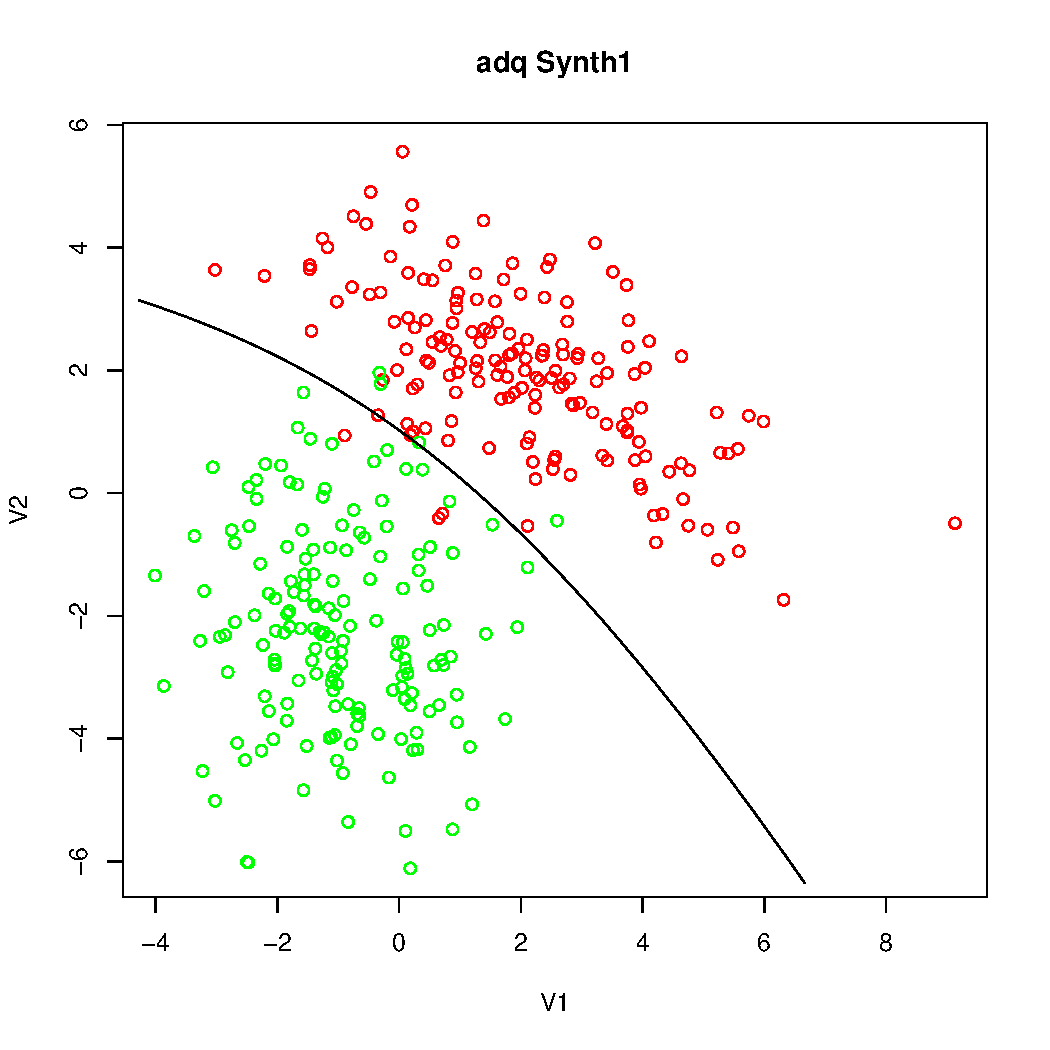
\includegraphics[width=0.7\textwidth]{results/adq/adq-Synth1.pdf}
    \caption{Frontières de décision de l'ADQ sur le dataset Synth1}
\end{center}
\end{figure}

\begin{figure}[ht!]
\begin{center}
    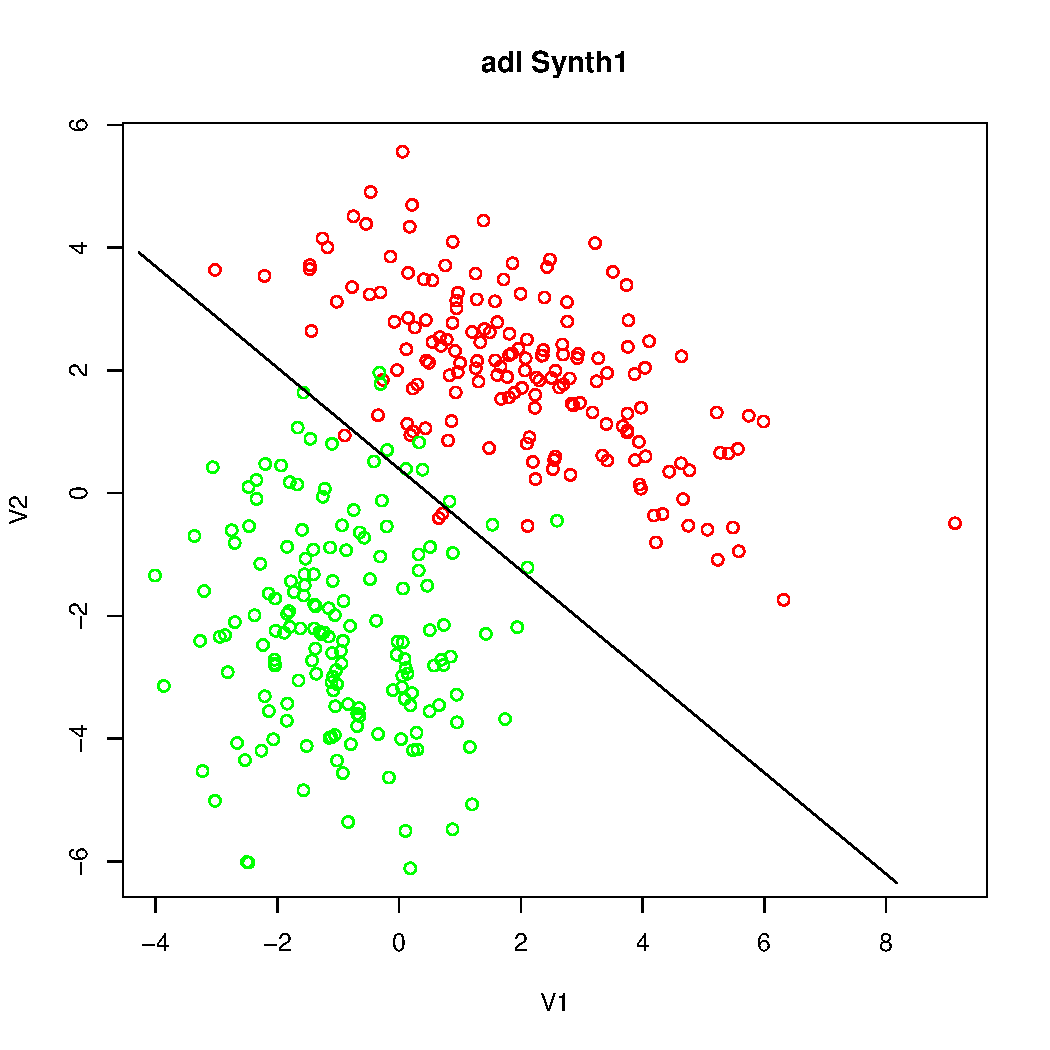
\includegraphics[width=0.6\textwidth]{results/adl/adl-Synth1.pdf}
    \caption{Frontières de décision de l'ADL sur le dataset Synth1}
\end{center}
\end{figure}

\begin{figure}[ht!]
\begin{center}
    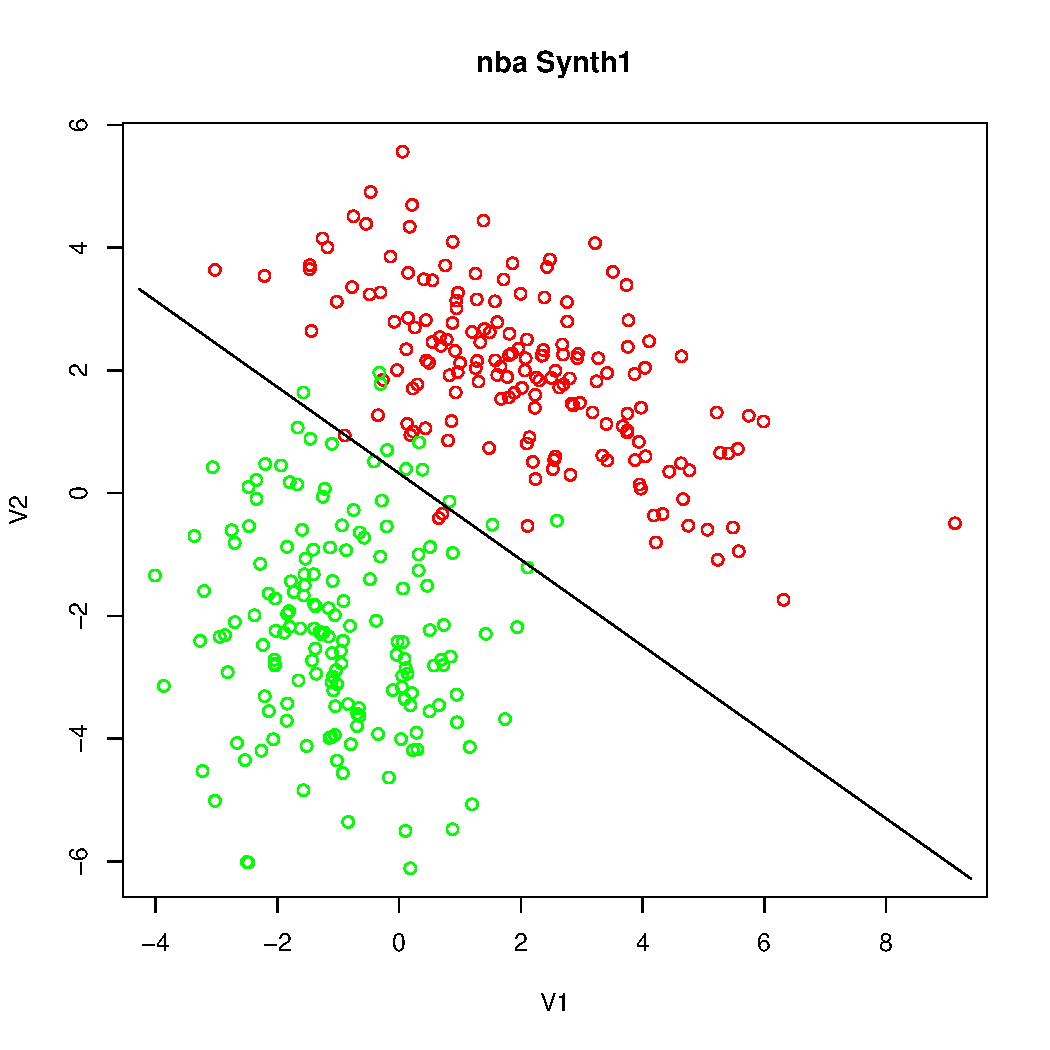
\includegraphics[width=0.6\textwidth]{results/nba/nba-Synth1.pdf}
    \caption{Frontières de décision du NBA sur le dataset Synth1}
\end{center}
\end{figure}

\begin{figure}[ht!]
\begin{center}
    \includegraphics[width=0.6\textwidth]{results/binlrt/binlrt-Synth1.pdf}
    \caption{Frontières de décision de la LOGBT sur le dataset Synth1}
\end{center}
\end{figure}

\begin{figure}[ht!]
\begin{center}
    \includegraphics[width=0.6\textwidth]{results/binlrf/binlrf-Synth1.pdf}
    \caption{Frontières de décision de la LOGBF sur le dataset Synth1}
\end{center}
\end{figure}

\begin{figure}[ht!]
\begin{center}
    \includegraphics[width=0.6\textwidth]{results/quadlrt/quadlrt-Synth1.pdf}
    \caption{Frontières de décision de la LOGQT sur le dataset Synth1}
\end{center}
\end{figure}

\begin{figure}[ht!]
\begin{center}
    \includegraphics[width=0.6\textwidth]{results/quadlrf/quadlrf-Synth1.pdf}
    \caption{Frontières de décision de la LOGQF sur le dataset Synth1}
\end{center}
\end{figure}


\clearpage
\paragraph{Interprétation}
A ce stade, difficile pour nous d'interpreter (sans comparaison possible). Notons tout de même le fait que la plupart des classifieurs ont un taux d'erreur relativement bas. Notons également que la différence entre ADL et NBA est très faible pour ce dataset. Notons finalement que le fait de rajouter une ordonnée à l'origine dans le cas de la Regression Logistique semble permettre au classifieur de mieux épouser la forme des classes à discriminer.

\newpage
\subsection{Synth2}
\paragraph{Résultats}
Le tableau ci-dessous récapitule les taux d'erreurs et intervalles de confiance de nos différents classifieurs sur le jeu de données \verb+Synth2+ :

\begin{table}[h!]
    \centering
    \caption{Estimations des taux d'erreurs et intervalles de confiances, par classifieur, sur le jeu de données "Synth2"}
    \label{tab:table1}
    \def\arraystretch{1.5}
    \begin{tabular}{c||c|c|c|c}
        \hline
        & ADQ & ADL & NBA & TREE\\
        \hline
        $\varepsilon$ & 0.011 & 0.012 & 0.015
        & 0.036\\
        \hline
        $IC$ & $[0.000 ; 0.022]$ & $[0.000 ; 0.023]$ & $[0.002 ; 0.029]$
        & $[0.016 ; 0.056]$\\
        \hline
        \hline
        & LOGBT & LOGBF & LOGQT & LOGQF\\
        \hline
        $\varepsilon$ & 0.013 & 0.014 & 0.014 & 0.013\\
        \hline
        $IC$ & $[0.000 ; 0.025]$ & $[0.001 ; 0.026]$ & $[0.001 ; 0.026]$ & $[0.001 ; 0.026]$\\
        \hline
        \hline
    \end{tabular}
\end{table}

\paragraph{Allures des frontières de décision}
Suivent ci-dessous le tracé des frontières de décision obtenues avec les différents classifieurs.

\begin{figure}[ht!]
\begin{center}
    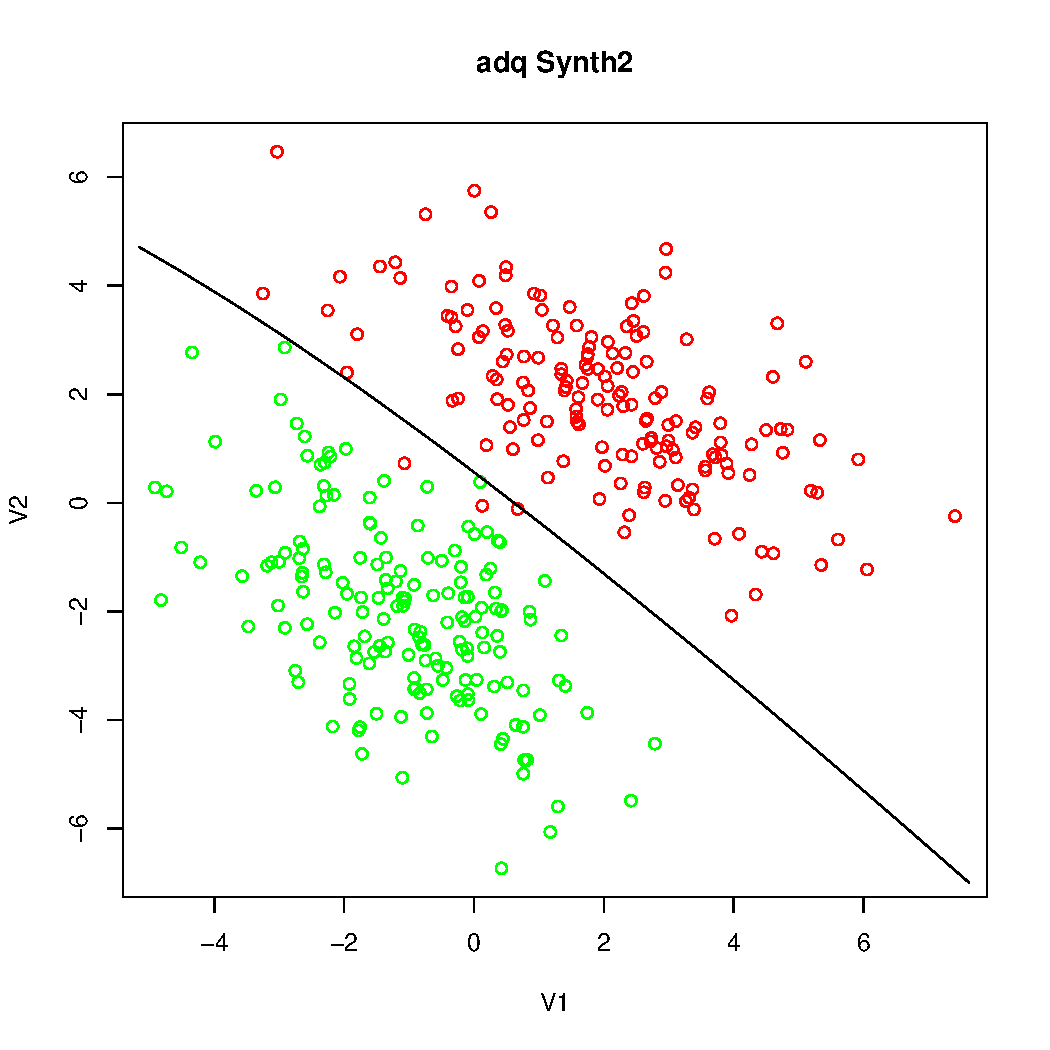
\includegraphics[width=0.7\textwidth]{results/adq/adq-Synth2.pdf}
    \caption{Frontières de décision de l'ADQ sur le dataset Synth2}
\end{center}
\end{figure}

\newpage
\begin{figure}[ht!]
\begin{center}
    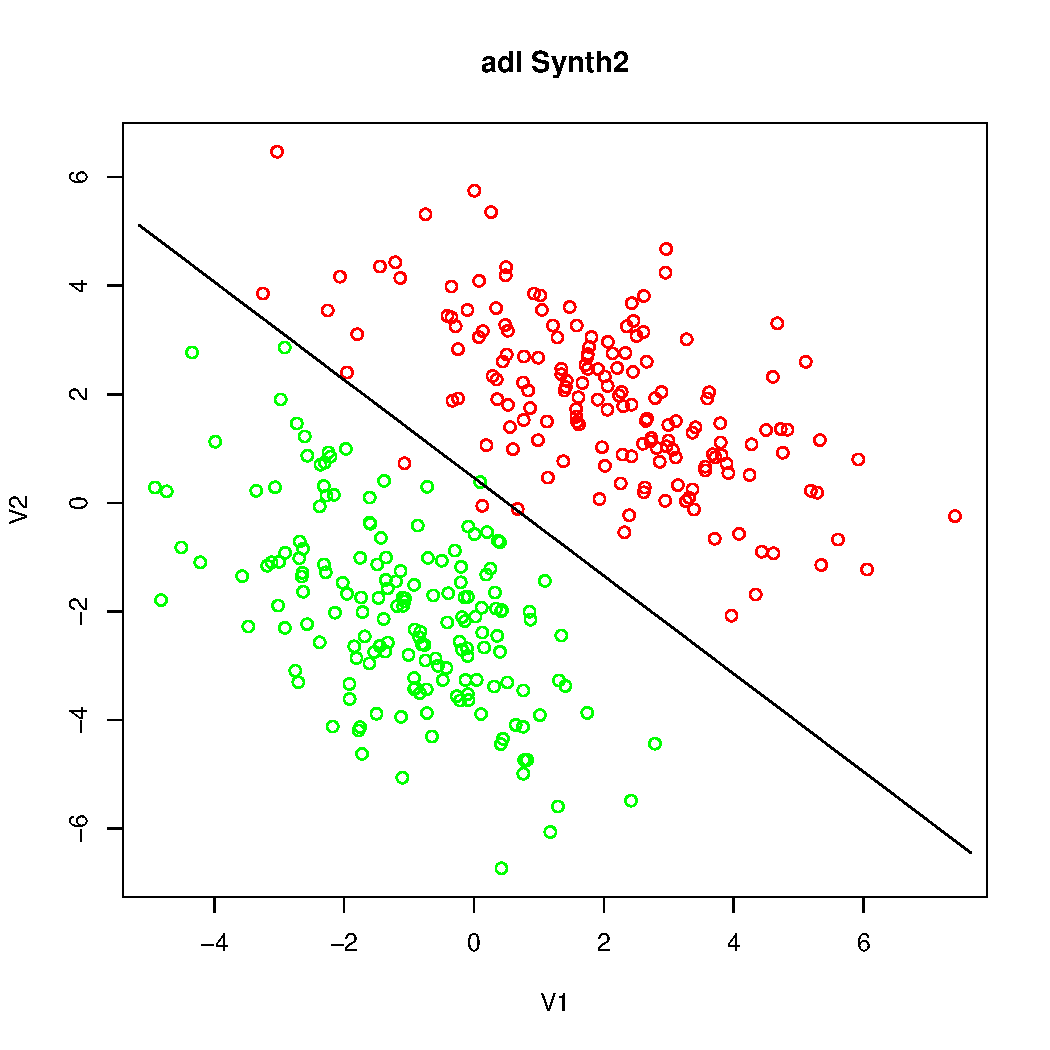
\includegraphics[width=0.6\textwidth]{results/adl/adl-Synth2.pdf}
    \caption{Frontières de décision de l'ADL sur le dataset Synth2}
\end{center}
\end{figure}

\begin{figure}[ht!]
\begin{center}
    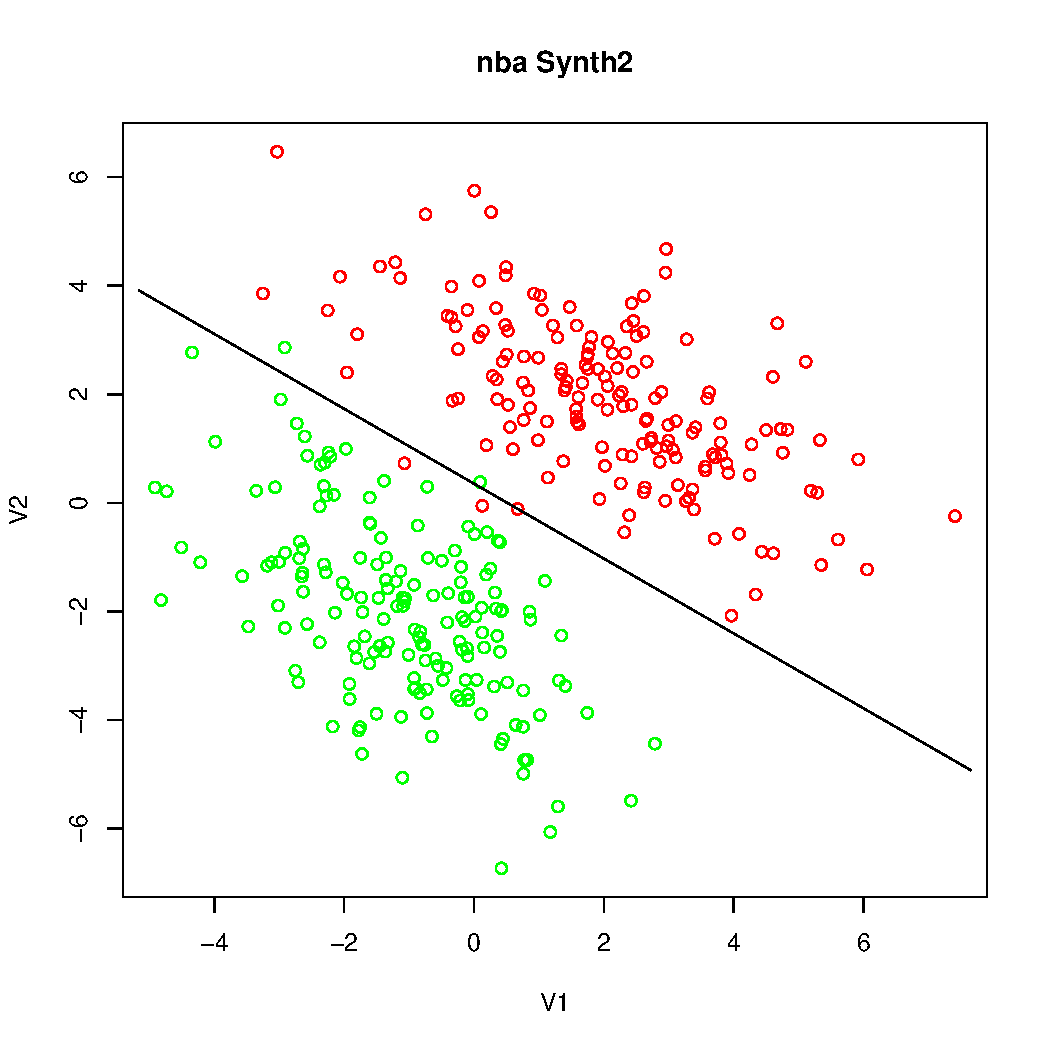
\includegraphics[width=0.6\textwidth]{results/nba/nba-Synth2.pdf}
    \caption{Frontières de décision du NBA sur le dataset Synth2}
\end{center}
\end{figure}

\begin{figure}[ht!]
\begin{center}
    \includegraphics[width=0.6\textwidth]{results/binlrt/binlrt-Synth2.pdf}
    \caption{Frontières de décision de la LOGBT sur le dataset Synth2}
\end{center}
\end{figure}

\begin{figure}[ht!]
\begin{center}
    \includegraphics[width=0.6\textwidth]{results/binlrf/binlrf-Synth2.pdf}
    \caption{Frontières de décision de la LOGBF sur le dataset Synth2}
\end{center}
\end{figure}

\begin{figure}[ht!]
\begin{center}
    \includegraphics[width=0.6\textwidth]{results/quadlrt/quadlrt-Synth2.pdf}
    \caption{Frontières de décision de la LOGQT sur le dataset Synth2}
\end{center}
\end{figure}

\begin{figure}[ht!]
\begin{center}
    \includegraphics[width=0.6\textwidth]{results/quadlrf/quadlrf-Synth2.pdf}
    \caption{Frontières de décision de la LOGQF sur le dataset Synth2}
\end{center}
\end{figure}

\clearpage
\paragraph{Interprétation}
Les performances de nos classifieurs issus de l'Analyse Discriminante comme de la Regression Logistique s'améliorent sur ce dataset. Seul l'Arbre de décision ne semble pas réellement progresser. Il semblerait que l'amélioration des performances de nos classifieurs reposant sur le calcul de probabilités à posteriori d'appartenance des individus au classes soit liée au fait que la séparation entre les deux classes est plus nette, le nombre d'outliers moins élevé permet de discriminer les individus de test à l'aide d'une frontière de décision qui en est plus pertinente.

\newpage
\subsection{Synth3}
\paragraph{Résultats}
Le tableau ci-dessous récapitule les taux d'erreurs et intervalles de confiance de nos différents classifieurs sur le jeu de données \verb+Synth3+ :

\begin{table}[h!]
    \centering
    \caption{Estimations des taux d'erreurs et intervalles de confiances, par classifieur, sur le jeu de données "Synth3"}
    \label{tab:table1}
    \def\arraystretch{1.5}
    \begin{tabular}{c||c|c|c|c}
        \hline
        & ADQ & ADL & NBA & TREE\\
        \hline
        $\varepsilon$ & 0.012 & 0.023 & 0.024
        & 0.042\\
        \hline
        $IC$ & $[0.000 ; 0.023]$ & $[0.007 ; 0.040]$ & $[0.007 ; 0.040]$
        & $[0.020 ; 0.064]$\\
        \hline
        \hline
        & LOGBT & LOGBF & LOGQT & LOGQF\\
        \hline
        $\varepsilon$ & 0.018 & 0.024 & 0.013 & 0.013\\
        \hline
        $IC$ & $[0.004 ; 0.033]$ & $[0.008 ; 0.041]$ & $[0.000 ; 0.025]$ & $[0.000 ; 0.025]$\\
        \hline
        \hline
    \end{tabular}
\end{table}

\paragraph{Allures des frontières de décision}
Suivent ci-dessous le tracé des frontières de décision obtenues avec les différents classifieurs.

\begin{figure}[ht!]
\begin{center}
    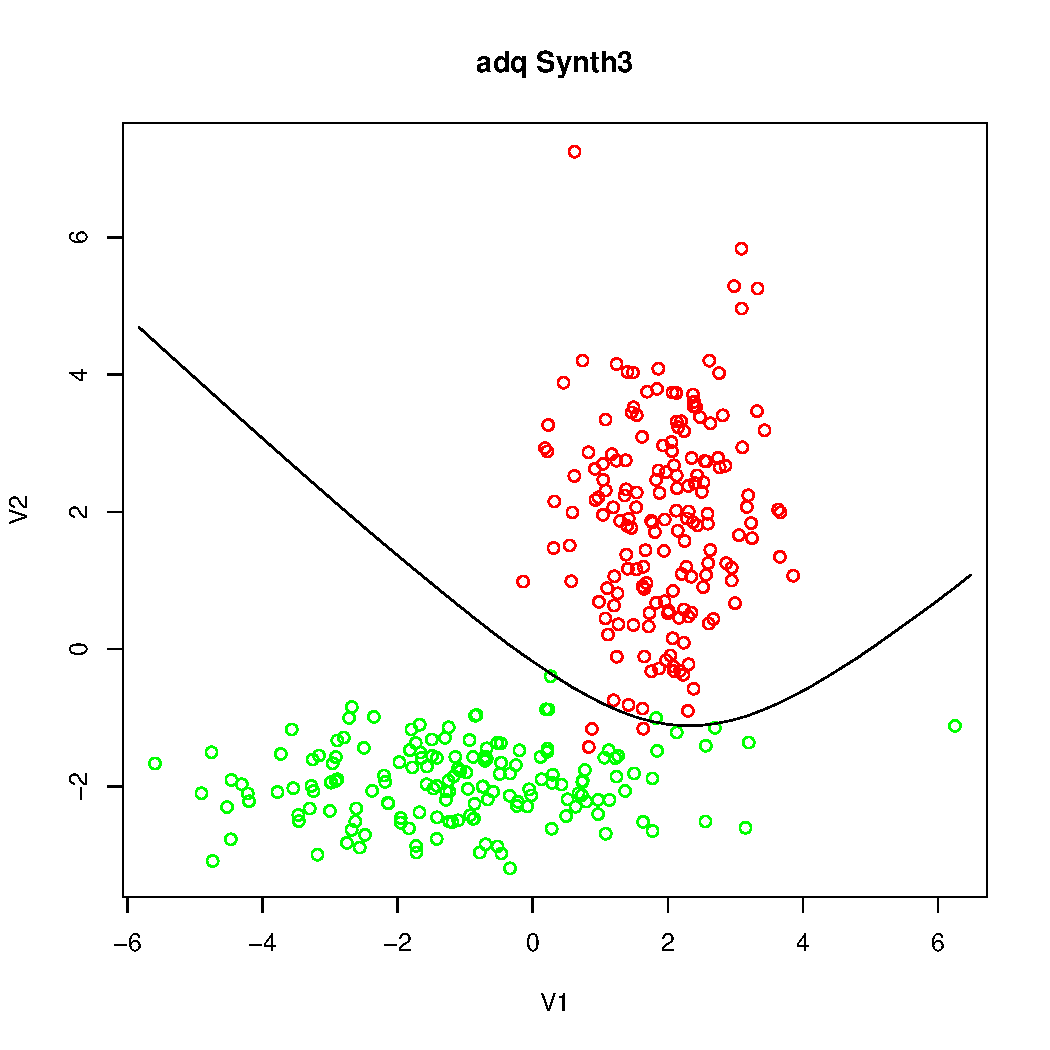
\includegraphics[width=0.7\textwidth]{results/adq/adq-Synth3.pdf}
    \caption{Frontières de décision de l'ADQ sur le dataset Synth3}
\end{center}
\end{figure}

\newpage
\begin{figure}[ht!]
\begin{center}
    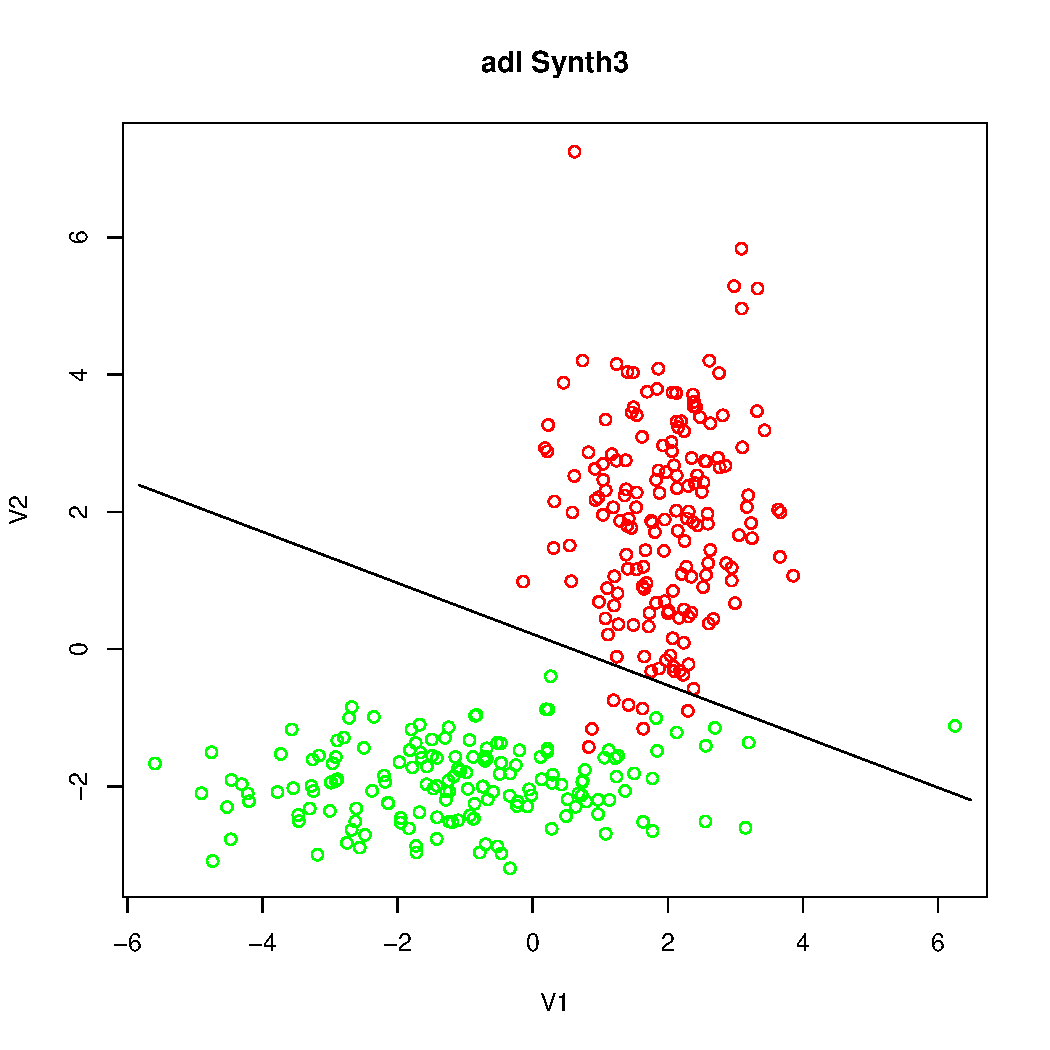
\includegraphics[width=0.6\textwidth]{results/adl/adl-Synth3.pdf}
    \caption{Frontières de décision de l'ADL sur le dataset Synth3}
\end{center}
\end{figure}

\begin{figure}[ht!]
\begin{center}
    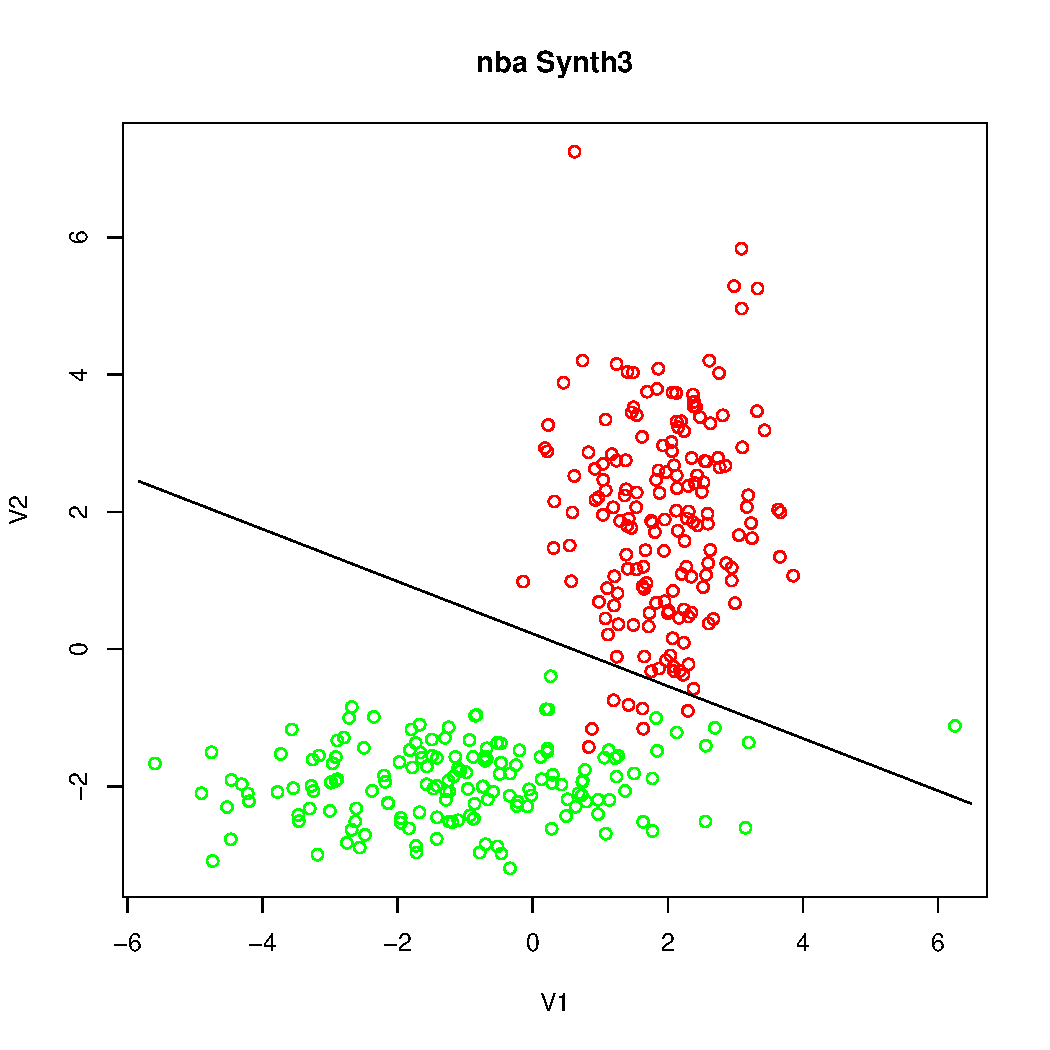
\includegraphics[width=0.6\textwidth]{results/nba/nba-Synth3.pdf}
    \caption{Frontières de décision du NBA sur le dataset Synth3}
\end{center}
\end{figure}

\begin{figure}[ht!]
\begin{center}
    \includegraphics[width=0.6\textwidth]{results/binlrt/binlrt-Synth3.pdf}
    \caption{Frontières de décision de la LOGBT sur le dataset Synth3}
\end{center}
\end{figure}

\begin{figure}[ht!]
\begin{center}
    \includegraphics[width=0.6\textwidth]{results/binlrf/binlrf-Synth3.pdf}
    \caption{Frontières de décision de la LOGBF sur le dataset Synth3}
\end{center}
\end{figure}

\begin{figure}[ht!]
\begin{center}
    \includegraphics[width=0.6\textwidth]{results/quadlrt/quadlrt-Synth3.pdf}
    \caption{Frontières de décision de la LOGQT sur le dataset Synth3}
\end{center}
\end{figure}

\begin{figure}[ht!]
\begin{center}
    \includegraphics[width=0.6\textwidth]{results/quadlrf/quadlrf-Synth3.pdf}
    \caption{Frontières de décision de la LOGQF sur le dataset Synth3}
\end{center}
\end{figure}

\clearpage
\paragraph{Interprétation}
Nous remarquons ici un écart de performances important entre l'ADQ d'une part, et l'ADL et le NBA d'autre part. Il semblerait qu'ici l'hypothèse d'homoscédasticité des données donne de bien moins bons résultats, ce qui nous laisse penser que le paramètre covariance utilisé pour générer chacune des classes est différent. Notons également la relative constance des résultats obtenus par les arbres de décision, en deça des performances de l'Analyse Discriminante et de la Regression Logistique, tout en restant respectable.

\newpage
\subsection{Pima}
\paragraph{Résultats}
Le tableau ci-dessous récapitule les taux d'erreurs et intervalles de confiance de nos différents classifieurs sur le jeu de données \verb+Pima+ :

\begin{table}[h!]
    \centering
    \caption{Estimations des taux d'erreurs et intervalles de confiances, par classifieur, sur le jeu de données "Pima"}
    \label{tab:table1}
    \def\arraystretch{1.5}
    \begin{tabular}{c||c|c|c|c}
        \hline
        & ADQ & ADL & NBA & TREE\\
        \hline
        $\varepsilon$ & 0.240 & 0.221 & 0.236
        & 0.267\\
        \hline
        $IC$ & $[0.177 ; 0.302]$ & $[0.160; 0.282]$ & $[0.174 ; 0.299]$
        & $[0.202 ; 0.332]$\\
        \hline
        \hline
        & LOGBT & LOGBF & LOGQT & LOGQF\\
        \hline
        $\varepsilon$ & 0.218 & 0.291 & 0.235 & 0.235\\
        \hline
        $IC$ & $[0.157 ; 0.279]$ & $[0.224 ; 0.358]$ & $[0.173 ; 0.297]$ & $[0.173 ; 0.297]$\\
        \hline
        \hline
    \end{tabular}
\end{table}

\paragraph{Interprétation}
Ce dataset est le premier dataset sur lequel nous éprouvons nos classifieurs sur des données réelles, et la première constatation qu'il nous est donné de faire est le fait que les performances de nos classifieurs sur des données réelles sont bien moins satisfaisantes. Le classifieur commettant le moins d'erreurs est la Regression Logistique binaire classique, avec ajout d'ordonnée à l'origine. Notons le gros écart de performances entre "ajout d'ordonnée à l'origine" et "sans ajout d'ordonnée à l'origine", semblant confirmer notre hypothèse précédente, selon laquelle l'ajout d'une ordonnée à l'origine est un choix intéressant, donnant une certaine liberté à notre frontière de décision, donc améliorant les performances de notre classifieur. L'autre fait marquant est le fait que parmis les trois modèles d'Analyse Discriminante, c'est l'ADL qui fourni les meilleures performances, suivie par le NBA, et enfin l'ADQ. Cela semble corroborer la théorie selon laquelle en diminuant le nombre de paramètre à estimer d'un modèle, on gagne en robustesse. Il est donc nécessaire de trouver le juste milieu, lors du choix des hypothèses d'un modèle, entre robustesse et spécificité du classifieur. Finalement, nous pouvons conclure ce paragraphe d'interprétation en émettant un doute sur le fait que nous sommes ici en présence de données rentrant tout à fait dans le schéma du "cas Gaussien", ce qui expliquerait les faibles performances de nos classifieurs reposant sur cette hypothèse.

\newpage
\subsection{BCW}
\paragraph{Résultats}
Le tableau ci-dessous récapitule les taux d'erreurs et intervalles de confiance de nos différents classifieurs sur le jeu de données \verb+BCW+ :

\begin{table}[h!]
    \centering
    \caption{Estimations des taux d'erreurs et intervalles de confiances, par classifieur, sur le jeu de données "BCW"}
    \label{tab:table1}
    \def\arraystretch{1.5}
    \begin{tabular}{c||c|c|c}
        \hline
        & ADQ & ADL & NBA\\
        \hline
        $\varepsilon$ & 0.052 & 0.045 & 0.039\\
        \hline
        $IC$ & $[0.024 ; 0.082]$ & $[0.018; 0.072]$ & $[0.014 ; 0.064]$\\
        \hline
        \hline
        & LOGBT & LOGBF & TREE\\
        \hline
        $\varepsilon$ & 0.039 & 0.158
        & 0.059\\
        \hline
        $IC$ & $[0.014 ; 0.064]$ & $[0.110 ; 0.205]$
        & $[0.028 ; 0.089]$\\
        \hline
        \hline
    \end{tabular}
\end{table}

\paragraph{Interprétation}
Ce dernier dataset produit de meilleurs résultats de la part de nos classifieurs. Peut être sommes nous de retour dans un cas se rapprochant plus du fameux "cas Gaussien" ? Cela expliquerait les bien meilleures performances de nos classifieurs. Nous remarquons directement que les classifieurs fournissant les meilleurs résultats sont ceux pour lesquels nous estimons le moins grand nombre de paramètre (NBA, Regression Logistique classique...) : nous pouvons émettre l'hypothèse que leurs meilleures performances est liée à leur meilleure robustesse présumée. Notons également les mauvaises performances de la Regression Logistique classique sans ajout d'ordonnée à l'origine, comparée aux autres classifieurs, qui semble une nouvelle fois confirmer la nécessité de cet ajout.

\newpage
\section{Conclusion}
\paragraph{Interprétations \& Conclusions}
De ces nombreux tests, nous tirons un certain nombre d'enseignements :
\begin{itemize}
    \item \textbf{Regression Logistique et ajout d'ordonnée à l'origine} : Il semble que l'ajout de cette fameuse ordonnée à l'origine soit un choix intéressant, pour donner plus de liberté à notre frontière de décision, et lui permettre ainsi de mieux épouser les différentes classes à discriminer.
    \item \textbf{Hypothèses et choix des classifieurs} : les performances d'un classifieur dépendra toujours des hypothèses que ce dernier assume comme vérifiées, et donc de la vérification de ces hypothèses au sein du jeu de données étudié. Il est donc nécessaire de trouver, pour chaque type de jeu de données, le classifieur le plus adapté, en émettant les bonnes hypothèses.
    \item \textbf{Robustesse contre spécificité} : Il est également nécessaire de trouver un certain juste milieu entre robustesse et spécificité, en prenant en compte le fait que généralement, plus on estime un grand nombre de paramètres lors de l'entrainement d'un classifieur, plus on perd en robustesse ce que l'on gagne en spécificité. Il est donc nécessaire de trouver le juste milieux, matchant au mieux nos besoins.
    \item \textbf{Evaluation des performances d'un classifieur} : L'estimation du risque des classifieurs envisagés, notamment grâce à des méthodes telles que la "méthode de l'ensemble de validation", la "validation croisée", ou encore le "bootstrap", est un bon indicateur des performances de chacun de ces derniers sur le jeu de données considéré.
\end{itemize}

\chapter{Conclusion}
\paragraph{Conclusion}
Ce TP a une nouvelle fois été l'occasion pour nous d'appliquer les connaissances théoriques concernants les différents classifieurs abordés en cours. Nous avons eu l'occasion d'implémenter et de tester l'Analyse Discriminante Quadratique, l'Analyse Discriminante Linéaire, le Classifieur Bayesien Naïf, la Regression Logistique classique, la Regression Logistique Quadratique, et pour finir les Arbres de décision. Nous permettant non seulement de consolider nos connaissances théoriques, ce TP a également été l'occasion de continuer nos progrès d'un point de vue technique, via les nombreuses heures passées devant notre écran à tenter de débuguer certains scripts légèrement récalcitrants. Finalement, ce TP nous a ouvert les yeux sur la nécessité de toujours se montrer précautionneux lorsqu'il s'agissait de choisir un modèle de classifieur (notamment pour les raisons abordées au sein de la conclusion de la partie précédente), ainsi que la nécessité d'en évaluer les performances avant de conclure sur sa pertinence.


\end{document}
